\documentclass[]{scrartcl}
\usepackage[letterpaper, margin = 1in, footskip = 0.25in]{geometry}
\usepackage{amsmath,amssymb,setspace,mathabx}
\usepackage{graphicx}
\usepackage{xcolor}
\usepackage{lscape}
\usepackage{verbatim}
\doublespacing

\providecommand{\tightlist}{%
  \setlength{\itemsep}{0pt}\setlength{\parskip}{0pt}}

% Redefine \includegraphics so that, unless explicit options are
% given, the image width will not exceed the width of the page.
% Images get their normal width if they fit onto the page, but
% are scaled down if they would overflow the margins.
\makeatletter
\def\ScaleIfNeeded{%
  \ifdim\Gin@nat@width>\linewidth
    \linewidth
  \else
    \Gin@nat@width
  \fi
}
\makeatother
\let\Oldincludegraphics\includegraphics
{%
 \catcode`\@=11\relax%
 \gdef\includegraphics{\@ifnextchar[{\Oldincludegraphics}{\Oldincludegraphics[width=\ScaleIfNeeded]}}%
}%

\setcounter{secnumdepth}{0}

\ifxetex
  \usepackage[setpagesize=false, % page size defined by xetex
              unicode=false, % unicode breaks when used with xetex
              xetex]{hyperref}
\else
  \usepackage[unicode=true]{hyperref}
\fi
\hypersetup{breaklinks=true,
            bookmarks=true,
            pdfauthor={},
            pdftitle={},
            colorlinks=true,
            citecolor=blue,
            urlcolor=blue,
            linkcolor=magenta,
            pdfborder={0 0 0}}
\urlstyle{same}  % don't use monospace font for urls


\author{}
\date{}


\begin{document}





\newpage

\section{Figures and Tables}\label{figures-and-tables}

\begin{landscape}
\begin{figure}[htbp]
\centering
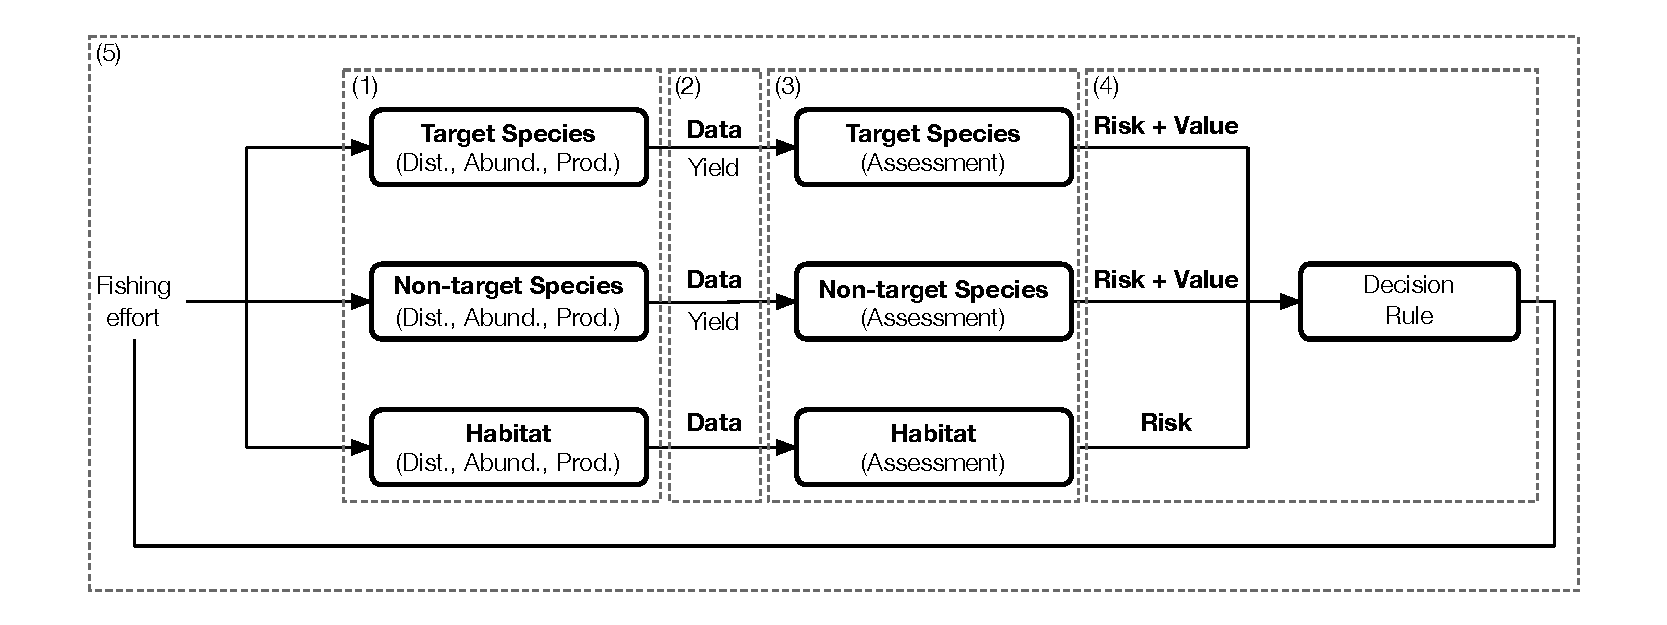
\includegraphics{figures/mscMSE.pdf}
\caption{A simplified fishery managment system divided into 5 discrete units. (1) Applied Population Ecology, (2) Fisheries Data Science, (3) Stock Assessment Modeling, (4) Risk Assessment, (5) Management Strategy Evaluation.}\label{fig:fishMgmt}
\end{figure}
\end{landscape}

\newpage

\begin{figure}[htbp]
\centering
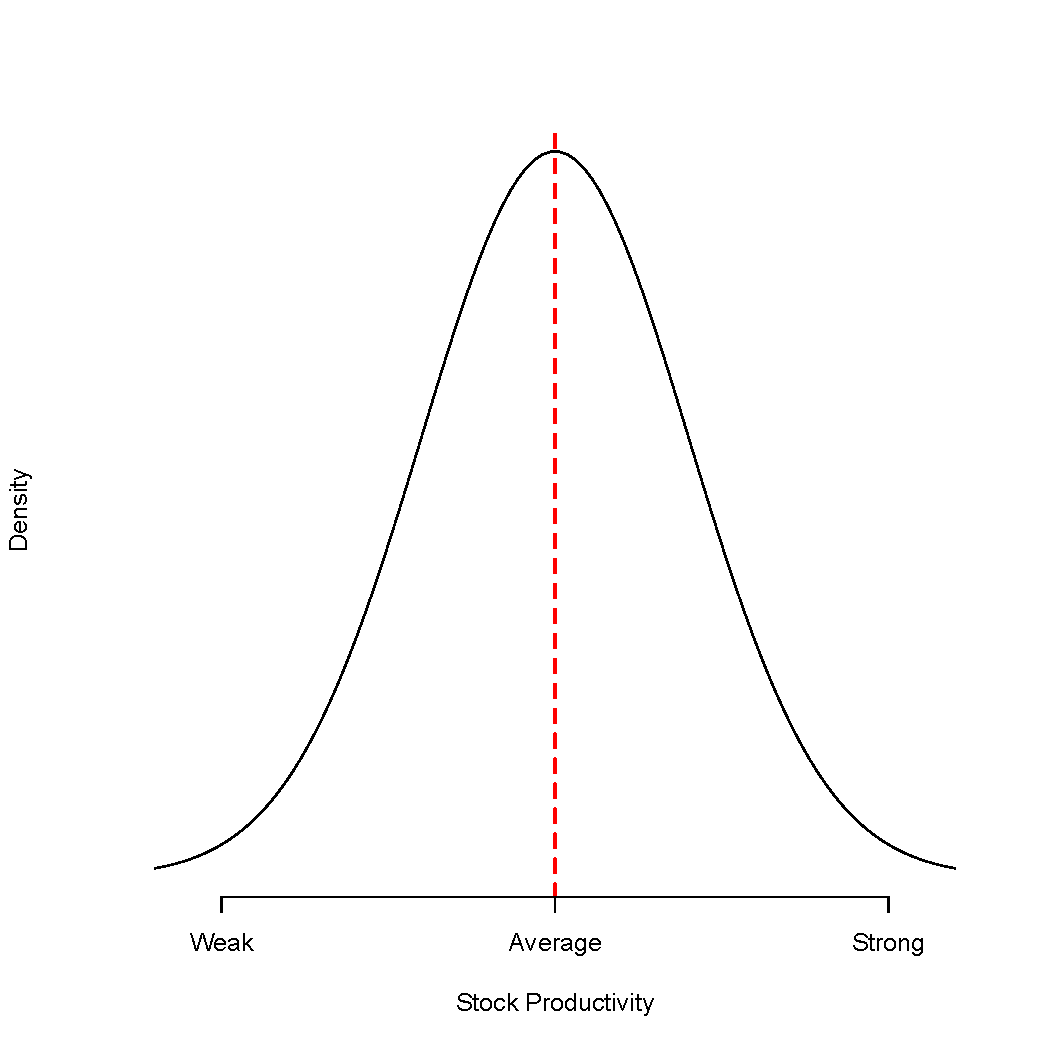
\includegraphics{figures/WeakStrongDist.pdf}
\caption{A conceptual model of the distribution of stock productivities in Pacific salmon. Harvesting according to the average productivity level leads to overfishing of the weakest stocks.}\label{fig:ppHCR}
\end{figure}

\newpage

\begin{figure}[htbp]
\centering
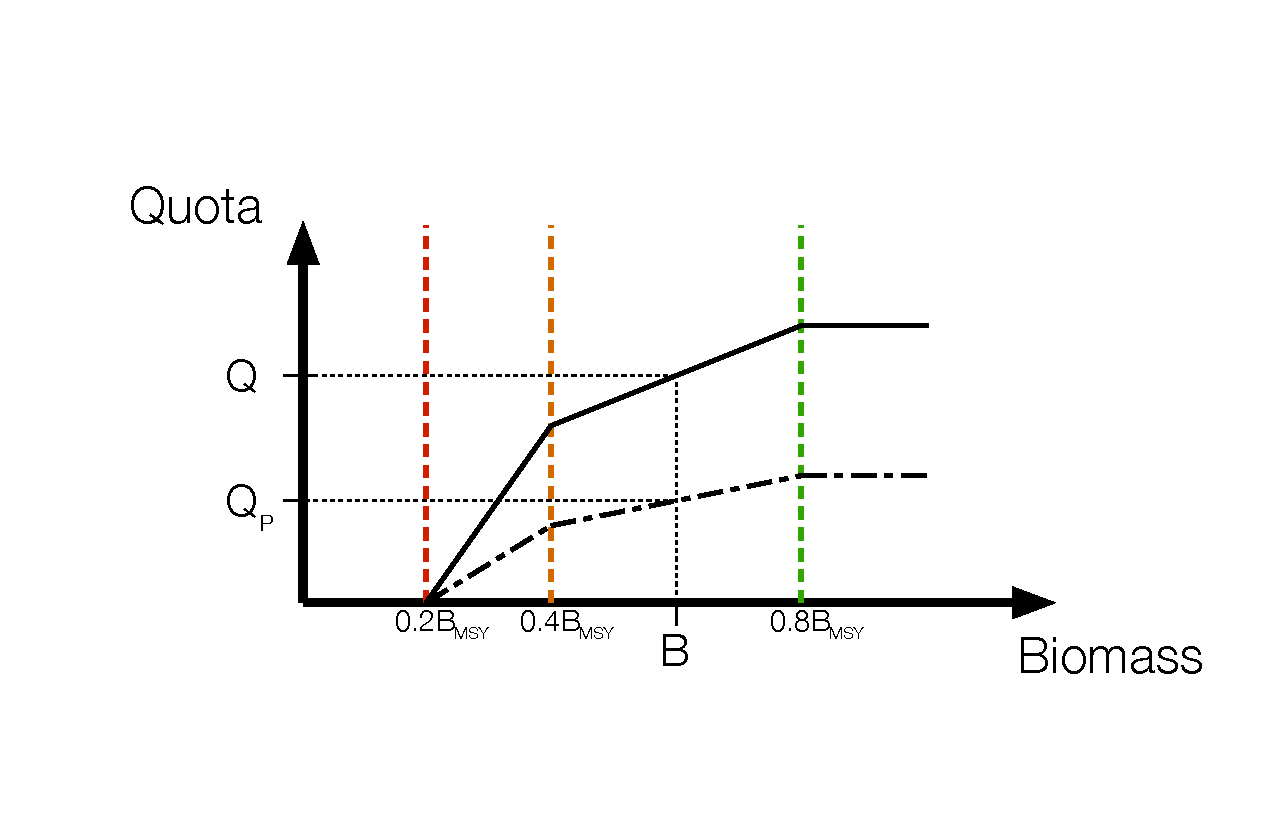
\includegraphics{figures/ppHCR.pdf}
\caption{A harvest control rule showing how the presence of pinch-point species affects the harvesting of directed species. The solid black line is the normal harvest control rule for a high productivity directed species, set by stock assessment, while the dashed black line shows the effective harvest control rule in the presence of technical interactions with pinch-point species. For a given stock biomass $B$ the directed species quota is $Q$, but pinch-point species reduce that to an effective or utilised quota of $Q_P$. The reduction in resources caused by the pinch-point species is then $Q - Q_P$.}\label{fig:ppHCR}
\end{figure}

\newpage

\begin{figure}[htbp]
\centering
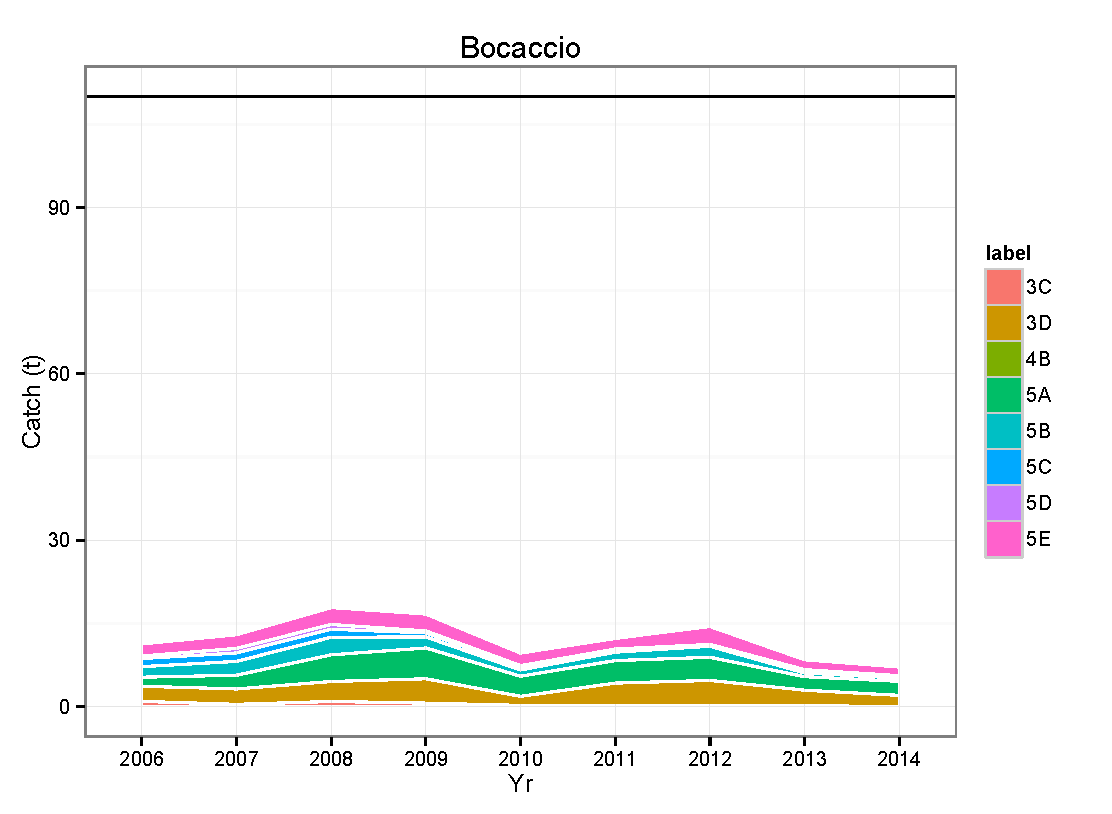
\includegraphics{figures/bocaccio.pdf}
\caption{Quota utilisation of Bocaccio rockfish in the BC integrated groundfish fishery. The black line represents the average annual total allowable catch (taken from the Pacific Region Integrated Fishery Management Plan) and the coloured polygons represent the biomass of removals in each management area.}\label{fig:bocaccio}
\end{figure}

\newpage

\begin{figure}[htbp]
\begin{center}
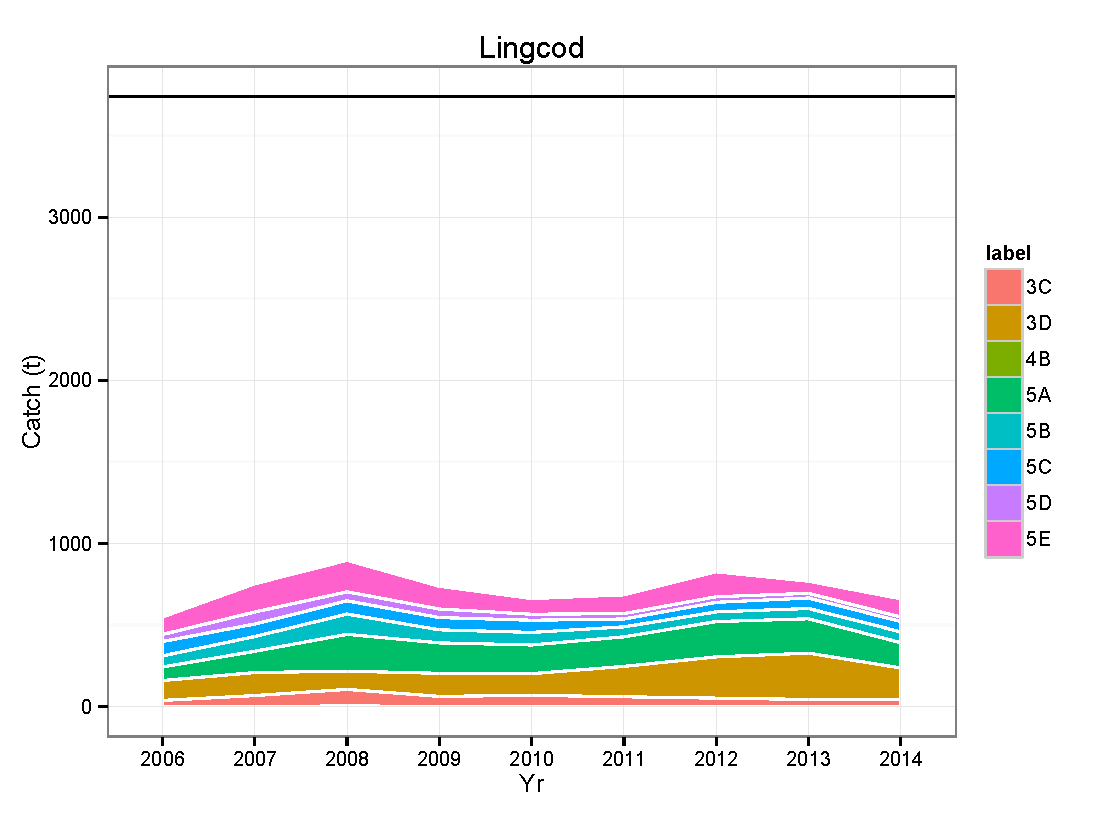
\includegraphics{figures/lingcod.pdf}
\caption{Quota utilisation of lingcod in the BC integrated groundfish fishery. The black line represents the average annual total allowable catch (taken from the Pacific Region Integrated Fishery Management Plan) and the coloured polygons represent the biomass of removals in each management area.}\label{fig:lingcod}
\end{center}
\end{figure}

\newpage

\begin{landscape}
\begin{figure}[htbp]
\begin{center}
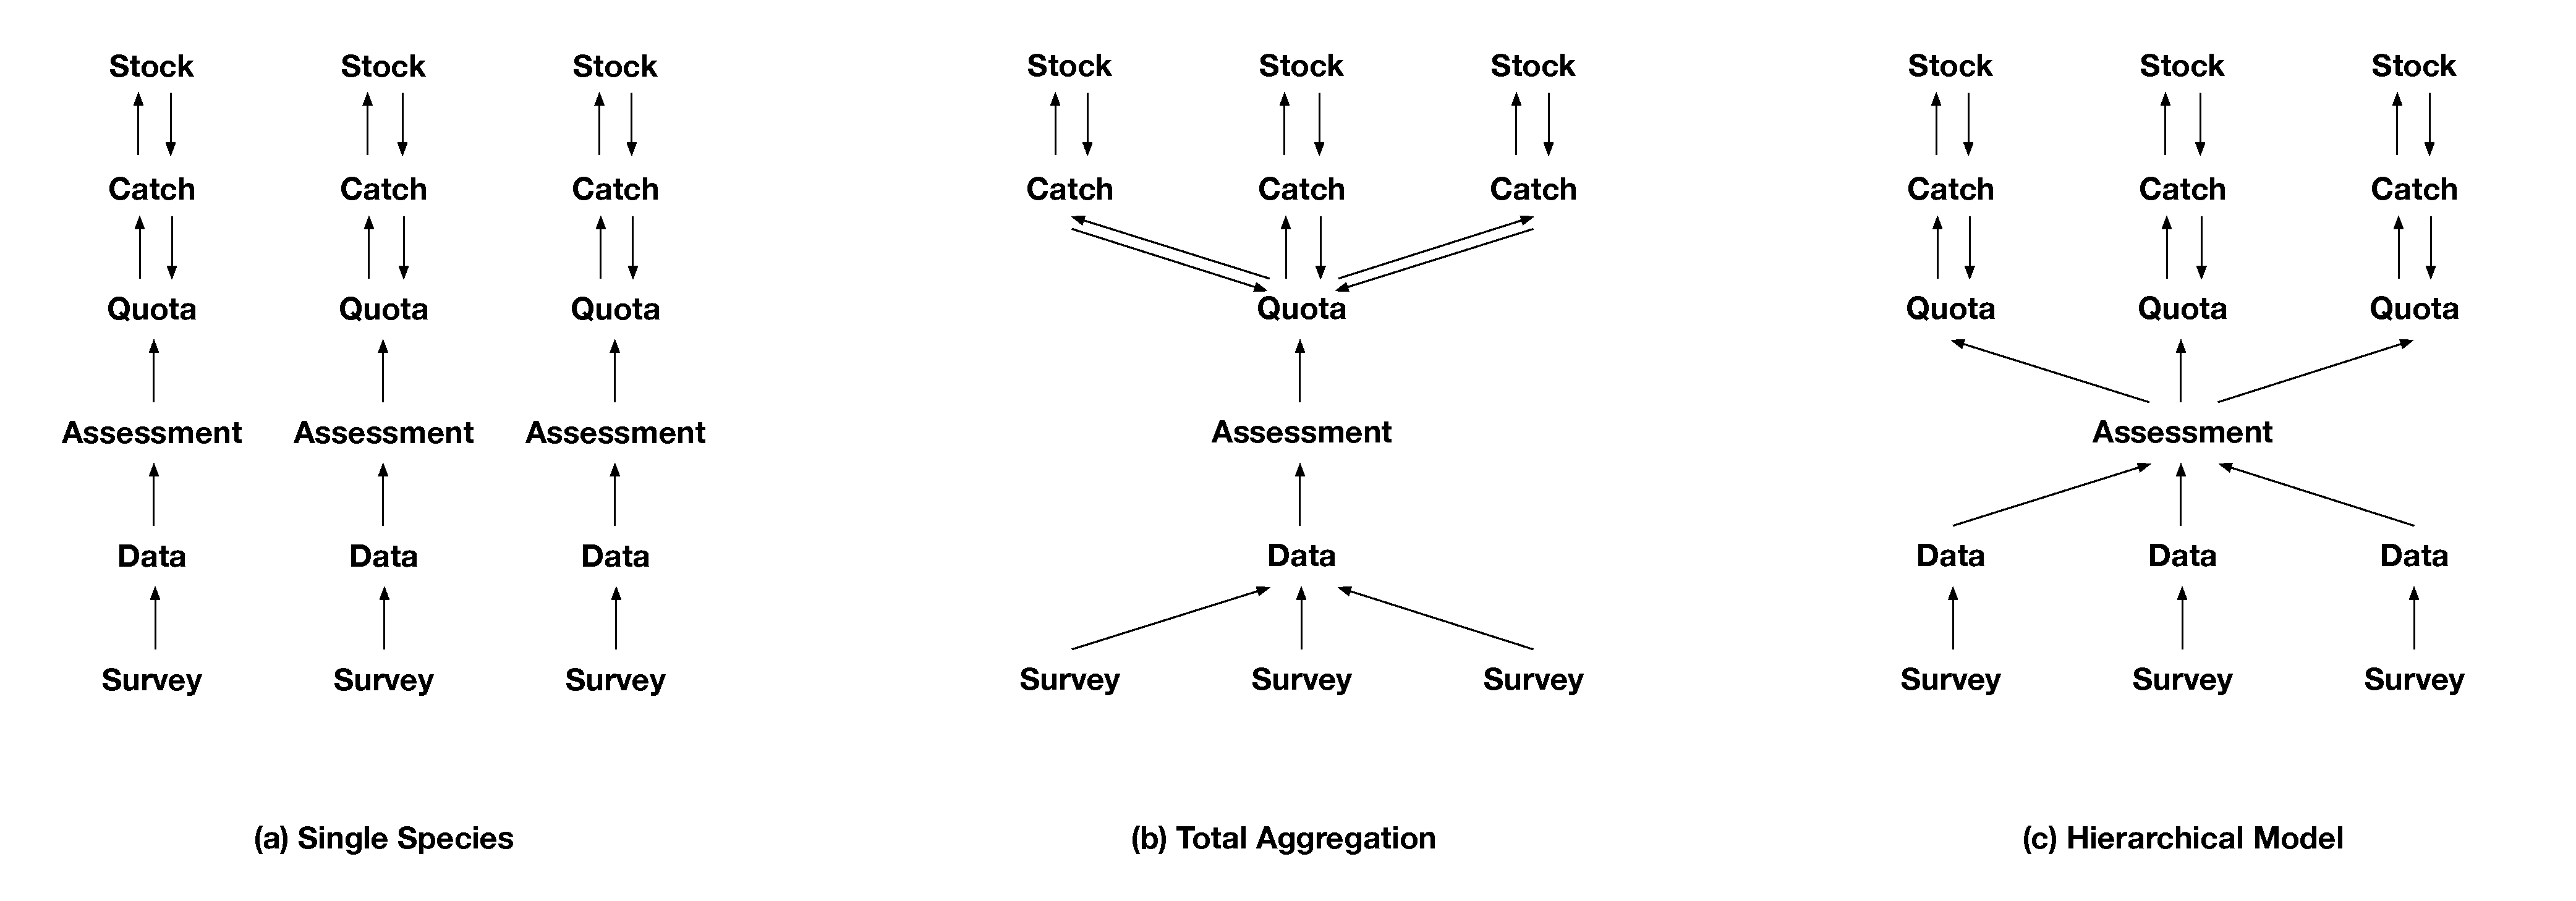
\includegraphics{figures/msFishery.pdf}
\caption{Three models of fishery management: (a) status quo,
single species approach; (b) hierarchical multi-species model; (c) total aggregation of species}\label{fig:3Models}
\end{center}
\end{figure}
\end{landscape}

\newpage

\begin{table}[htbp]
\begin{center}
\caption{Variable definitions for simulation and estimation of a multispecies fishery with no substock structure used in Chapter 1. The population dynamics are driven by a simple Biomass Dynamics model (Hilborn and Walters, 1992, Ch, 8). Catch is dependent on fishing mortality for each species, which is an input to the model. The current specification can be considered to be "coastwide" in the sense that it aggregates all discrete stocks of each species into a single management unit.}\label{tab:Ch1spec}
\begin{tabular}{c|l}
\textit{Variable} & \textit{Description}  \\
\hline
& \textbf{ Index Variables} \\
\hline
$S$ & Total number of species \\
$F$ & Total number of fleets \\
$T$ & Total number of years \\
$s$ & Species index \\
$f$ & Fleet index \\
$t$ & Time index \\
\hline
& \textbf{ Biological Model} \\
\hline
$B_{s,t}$ & Biomass of species $s$ at time $t$ \\
$B_{s,0}$ & Unfished biomass of species $s$ \\
$r_{s}$ & Average intrinsic rate of growth for speces $s$ \\
\hline
& \textbf{ Observation Model} \\
\hline
$q_{s}$ & Survey catchability of species $s$ \\
$I_{s,t}$ & Fishery independent CPUE of species $s$ at time $t$ \\
\hline
& \textbf{ Output (catch) } \\
\hline
$F_{s,t}$ & Fishing mortality of species $s$ at time $t$ \\
$C_{s,t}$ & Catch of species $s$ at time $t$ \\
\hline
& \textbf{ Stochastic Model} \\
\hline
$\Sigma$ & Species specific process error covariance matrix  \\
$\zeta_t = \left(\zeta_{s,t}\right)_{s=1}^S$ & Vector of species specific process errors $\left(\zeta_t \sim N ( \vec{0}, \Sigma)\right)$  \\
$\sigma^2$ & Coastwide environmental process error variance \\
$\epsilon_{t}$ & Coastwide environmental process error at time $t$, $\left( \epsilon_{t} \sim N (0, \sigma^2) \right)$ \\
$\tau_s^2$ & Observation error variance for species $s$ \\
$\delta_{s,t}$ & Observation error for species $s$ at time $t$ $\left(\epsilon_{s,t} \sim N (0, \tau_s^2) \right)$ \\
$\overline{\log q}$ & Shared multispecies prior mean on $\log$ catchability \\
$\kappa^2$ & Multispecies prior variance on $\log$ catchability \\
\hline
\end{tabular}
\end{center}
\end{table}

\newpage

\begin{table}[htbp]
\begin{center}
\caption{The simulation model to produce data for the estimation procedure in Chapter 1. The simulator generates time series of catch, biomass and CPUE for species $s$ with input parameters $\Theta_s$. All variables are defined in Table \ref{tab:Ch1spec}. The notation $\Sigma_{(s)}$ refers to the entry on the main diagonal corresponding to species $s$.}\label{tab:Ch1sim}
\begin{tabular}{cl}
\hline
& \textbf{Simulation Parameters} \\
(T2.1) & $\Theta_s = \left( B_{s,0}, r_s, q_s, 
                          \{F_{s,t}\}_{t = 1}^{T},
                          \Sigma, \sigma_s^2, \tau_s^2 \right)$ \\
& \\
& \textbf{ Initial States ($t = 1$) } \\
(T2.2) & $B_{s,1} = B_{s,0} \cdot e^{(\zeta_{s,1} - \Sigma_{(s)}/2) + (\epsilon_1 - \sigma^2/2)}$ \\
& \\
& \textbf{ Catch ($1 \leq t \leq T$) } \\
(T2.3) & $C_{s,t} = \left(1 - e^{F_{s,t}}\right)\cdot B_{s,t}$ \\
& \\
& \textbf{ State Dynamics ($2 \leq t \leq T$)} \\
(T2.4) & $B_{s,t} = \left ( B_{s,t-1} + r_sB_{s,t-1}\left( 1 - \frac{B_{s,t-1}}{B_{s,0}} \right) - C_{s,{t-1} } \right) \cdot e^{(\zeta_{s,t} - \Sigma_{(s)}/2) + (\epsilon_t - \sigma^2/2)}$ \\
& \\
& \textbf{ Observations ($1 \leq t \leq T$)} \\
(T2.5) & $I_{s,t} = q_s \cdot B_{s,t} \cdot e^{\delta_{s,t} - \tau_s^2/2}$ \\
\hline
\end{tabular}
\end{center}
\end{table}

\newpage

\begin{table}[htbp]
\caption{Selected elements of the hierarchical stock assessment model used as the estimation procedure Chapter 1. The function $f_s(\Theta_s)$ in the species specific posterior density (T3.10) represents the species specific prior distributions that are omitted from the table. The notation $\Sigma^{(S)}_{(s)}$ refers to the entry on the main diagonal of $\Sigma^{(S)}$ corresponding to species $s$.}\label{tab:Ch2est}
\begin{center}
\begin{tabular}{cl}
\hline
& \textbf{Assessment Parameters} \\
(T3.1) & $\Theta_s = \left\{ B_{s,0}, r_s, q_s, 
                            \tau_s^2, \Sigma,
                            \left\{ I_{s,t} \right\}_{t = 1}^T,
                            \left\{ C_{s,t} \right\}_{t = 1}^T \right\}$ \\
(T3.2) & $\Theta = \left\{ \left\{\Theta_s) \right\}_{s = 1}^S, \sigma^2, \log q, \kappa^2 \right\}$ \\
& \\
& \textbf{ Population Dynamics Model } \\
(T3.3) & $B_{s,1} = B_{s,0} \cdot e^{(\zeta_{s,1} - \Sigma_{(s)}^2/2) + (\epsilon_1 - \sigma^2/2)}$ \\
(T3.4) & $B_{s,t} = \left ( B_{s,t-1} + r_sB_{s,t-1}\left( 1 - \frac{B_{s,t-1}}{B_{s,0}} \right) - C_{s,{t-1} } \right) \cdot e^{(\zeta_{s,t} - \Sigma_{(s)}^2/2) + (\epsilon_{t} - \sigma^2/2)}$,~~~ $2 \leq t \leq T$, \\
& \\
& \textbf{ Observational Model ($1 \leq t \leq T$)} \\
(T3.5) & $\overline{I_{s,t}} = q_s \cdot B_{s,t} \cdot e^{\delta_{s,t} - \tau_s^2/2}$ \\
& \\
& \textbf{ Statistical Model } \\
& \textit{ Data Likelihood } \\
(T3.6) &  $\mathcal{L}_s \left( \left\{ I_{s,t} \right\}_{t = 1}^T ~|~
                                \Theta_s \right) \sim \log N \left( \left\{ \overline{I_{s,t}} \right\}_{t = 1}^T, \tau_s^2 \right)$ \\
& \textit{ Multispecies Prior Distributions } \\
(T3.7) &  $p \left( \epsilon_{t} ~|~ \sigma^2 \right) = N \left( 0, \sigma^2\right)$\\
(T3.8) &  $p \left( \zeta_{t} ~|~ \Sigma \right) = N \left( \vec{0}, \Sigma \right)$\\
(T3.9) & $p \left( \log q_s ~|~ \overline{\log q}, \kappa^2 \right) \sim N \left( \overline{\log q}, \kappa^2 \right)$ \\
& \textit{ Posterior Density } \\
(T3.10) & $\mathcal{P}_s = \mathcal{L}_s \cdot p \left( \log q_s ~|~ \overline{\log q}, \kappa^2 \right) \cdot f_s(\Theta_s)$ \\
(T3.11) & $\mathcal{P} = \prod_{s = 1}^S \mathcal{P}_s \cdot
            \prod_{t = 1}^T \left( p \left( \epsilon_{t} ~|~ \sigma^2 \right) \cdot p \left( \zeta_{t} ~|~ \Sigma \right) \right ) 
             $ \\
\hline
\end{tabular}
\end{center}
\end{table}

\newpage

\begin{figure}[htbp]
\centering
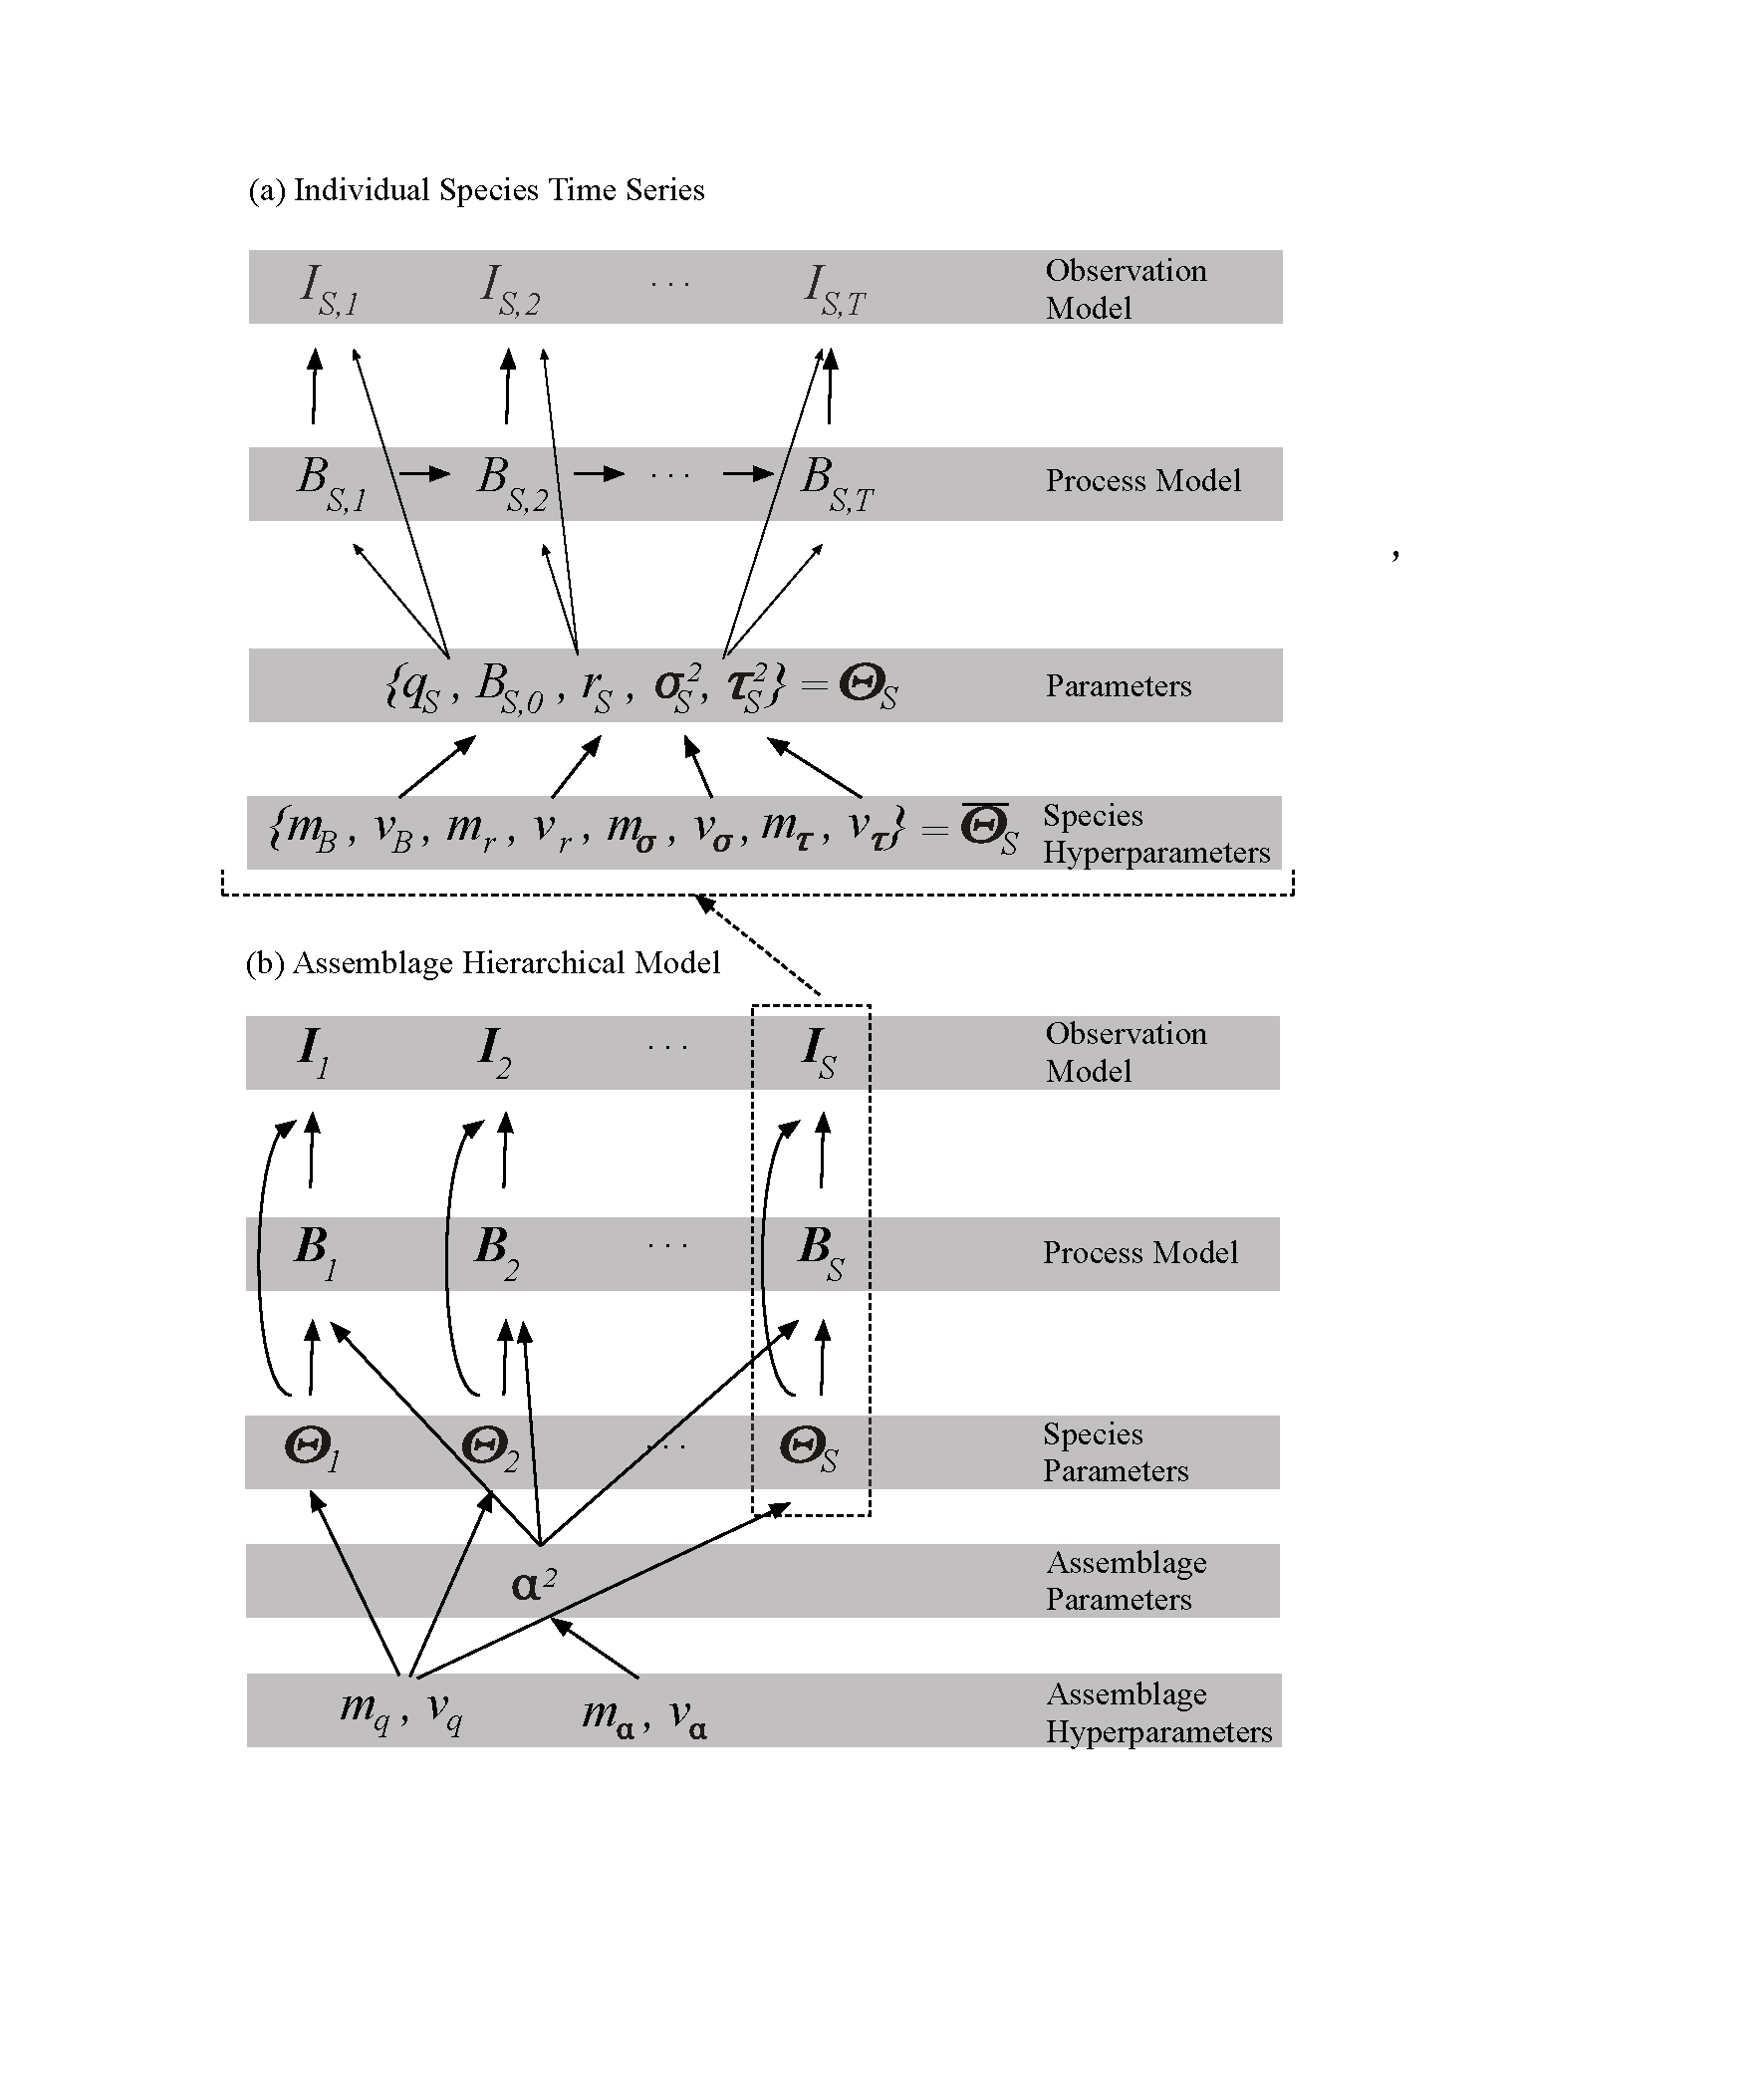
\includegraphics{figures/HBMClarkCh1.pdf}
\caption{A conceptual diagram of the hierarchical model used for estimation in Chapter 1.  Part (a) shows the individual species process and observation models, with species specific parameters and hyperparameters. Part (b) compresses the time series into bold italicised variables, and shows the hierarchically arranged multispecies assemblage with shared multispecies parameters and hyperparameters.}\label{fig:HBMCh1}
\end{figure}

\newpage

\begin{figure}[htbp]
\centering
\includegraphics{figures/Ft.pdf}
\caption{Three instantaneous fishing mortality $F_t$ trends over 40 years of management history. The black line shows a steady linear increase over the time period to a (fully selected) maximum of $F_t = 1$. The red line shows a fishery that developed over 20 years and then held fishing mortality steady at $F_t = 1$ for the following 20. Both trajectories correspond to developmental periods of a fishery, which provides little information about a stock's response to alleviating fishing pressure. Finally, the blue line shows a more informative sawtooth pattern, with periods of increasing and decreasing fishing pressure over the 40 year management period. Here, stock dynamics will respond to the changes in fishing pressure and provide more information about productivity than the other two cases.}\label{fig:HBMCh1}
\end{figure}

\newpage

\begin{table}[htbp]
\begin{center}
\caption{Variable definitions for simulation and estimation of a multispecies spatially structured multistock fishery used in Chapter 2. The population dynamics are driven by a simple Biomass Dynamics model (Hilborn and Walters, 1992, Ch, 8), with immigration and emigration between stocks of a species summarised by a migration rate $\phi_{s,p,p'}$. Catch is determined by instantaneous fishing mortality for each individual stock, which is defined as an input to the model.}\label{tab:Ch2spec}
\begin{tabular}{c|c}
\textit{Variable} & \textit{Description}  \\
\hline
& \textbf{ Index Variables} \\
\hline
$s$ & Species index \\
$p$ & Stock index \\
$f$ & Fleet index \\
$t$ & Time index \\
$S$ & Total number of species \\
$P_s$ & Total number of stocks of species s \\
$F$ & Total number of fleets \\
$T$ & Total number of years \\
\hline
& \textbf{ Biological Model} \\
\hline
$B_{s,p,t}$ & Biomass of stock $p$ of species $s$ at time $t$ \\
$B_{s,p,0}$ & Unfished biomass of stock $p$ of species $s$ \\
$r_{s,p}$ & Intrinsic rate of growth for stock $p$ of speces $s$ \\
$\phi_{s,p,p'}$ &  Net migration rate between stocks $p$ and $p'$ of species $s$ \\
\hline
& \textbf{ Observation Model} \\
\hline
$q_{s,p}$ & Survey catchability of stock $p$ of species $s$ at time $t$ \\
$I_{s,p,t}$ & Fishery independent CPUE of stock $p$ of species $s$ at time $t$ \\
\hline
& \textbf{ Catch} \\
\hline
$F_{s,p,t}$ & Fishing mortality of stock $p$ of species $s$ at time $t$ \\
$C_{s,p,t}$ & Total catch of stock $p$ of species $S$ at time $t$ \\
\hline
& \textbf{ Stochastic Model } \\
\hline
$\Sigma^{(P)}$ & Stock specific process error covariance matrix \\
$\xi_{t} = \left( \xi_{s,p,t} \right)_{(s,p) = (1,1)}^{(S,P)}$ & Vector of stock specific process errors at time $t$, $\left( \xi_t \sim N (\vec0, \Sigma^{(P)}) \right)$ \\
$\Sigma^{(S)}$ & Species specific process error covariance matrix \\
$\zeta_t = \left(\zeta_{s,t}\right)_{s=1}^S$ & Vector of species specific process errors $\left(\zeta_t \sim N ( \vec{0}, \Sigma)\right)$  \\
$\sigma^2$ & Coastwide process error variance \\
$\epsilon_{t}$ & Coastwide process error deviation at time $t$, $\left( \epsilon_{t} \sim N (0, \sigma^2) \right)$ \\
$\tau_{s,p}^2$ & Observation error variance for stock $p$ of species $s$ \\
$\delta_{s,p,t}$ & Observation error for stock $p$ of species $s$ at time $t$ $\left(\epsilon_{s,p,t} \sim N (0, \tau_s^2) \right)$ \\
$\overline{\log q_s}$ & Species specific prior mean on stock specific $\log$ catchability \\
$\kappa_s^2$ & Species specific prior variance for stock specific $\log$ catchability \\
$\overline{\log q}$ & Multispecies prior mean on species specific mean $\log$ catchability \\
$\kappa^2$ & Multispecies prior variance for species specific mean $\log$ catchability \\
$\overline{\log r_s}$ & Species specific prior mean on stock specific $\log$ intrinsic growth $r$ \\
$\rho_s^2$ & Species specific prior variance for stock specific $\log$ intrinsic growth $r$ \\
\hline
\end{tabular}
\end{center}
\end{table}

\newpage

\begin{table}[htbp]
\begin{center}
\caption{The simulation model to produce data for the estimation procedure in Chapter 2. The model generates time series of catch, biomass and CPUE for stock $j$ of species $s$ with input parameters $\Theta_s$. All variables are defined in Table \ref{tab:Ch2spec}. The notation $\Sigma^{(S)}_{(s)}$ refers to the entry on the main diagonal of $\Sigma^{(S)}$ corresponding to species $s$, with the analagous definition for $\Sigma^{(P)}_{(s,p)}$.}\label{tab:Ch2sim}
\begin{tabular}{cl}
\hline
& \textbf{Parameters} \\
(T5.1) & $\Theta_{s,j} = \left( B_{s,p,0}, r_{s,p}, q_{s,p}, 
                          \{ \phi_{s,p,p'} \}_{i \neq p},
                          \{F_{s,p,t}\}_{t = 1}^{T},
                          \Sigma^{(P)}, \Sigma^{(S)},
                          \sigma^2, \tau_{s,p}^2, T
                           \right)$ \\
& \\
& \textbf{ Initial States ($t = 1$) } \\
(T5.2) & $B_{s,p,1} = B_{s,p,0} \cdot e^{(\xi_{s,p,t} - \Sigma^{(P)}_{(s,p)}/2) + (\zeta_{s,t} - \Sigma^{(S)}_{(s)}/2) + (\epsilon_{t} - \sigma^2/2) }$ \\
& \\
& \textbf{ Catch ($1 \leq t \leq T$) } \\
(T5.3) & $C_{s,p,t} = \left(1 - e^{F_{s,p,t}}\right)\cdot B_{s,p,t}$ \\
& \\
& \textbf{ State Dynamics ($2 \leq t \leq T$)} \\
(T5.4) & $B_{s,p,t} = \left ( B_{s,p,t-1} + r_{s,p}B_{s,p,t-1}\left( 1 - \frac{B_{s,p,t-1}}{B_{s,0}} \right) + \sum_{p' \neq p} \phi_{s,p,p
'} \cdot B_{s,p',t-1} - C_{s,p,{t-1} } \right) \cdot$ \\ 
& ~~~~~~~~~~~~~~~~~~~~~~~~~$e^{(\xi_{s,p,t} - \Sigma^{(P)}_{(s,p)}/2) + (\zeta_{s,t} - \Sigma^{(S)}_{(s)}/2) + (\epsilon_{t} - \sigma^2/2)}$ \\
& \\
& \textbf{ Observation model ($1 \leq t \leq T$)} \\
(T5.5) & $I_{s,p,t} = q_{s,p} \cdot B_{s,p,t} \cdot e^{\delta_{s,p,t} - \tau_{s,p}^2/2}$ \\
\hline
\end{tabular}
\end{center}

\end{table}

\newpage

\begin{table}[htbp]
\begin{center}
\caption{A truncated version of the hierarchical stock assessment model used as the estimation procedure Chapter 2. The functions $f_{s,p}(\Theta_{s,p})$ and $f_s(\Theta_s)$ represent the stock and species specific prior distributions that were omitted from the table. All variables used here are defined in Table \ref{tab:Ch2spec}. The notation $\Sigma^{(S)}_{(s)}$ refers to the entry on the main diagonal of $\Sigma^{(S)}$ corresponding to species $s$, with the analagous definition for $\Sigma^{(P)}_{(s,p)}$}\label{tab:Ch2est}
\begin{tabular}{cl}
\hline
& \textbf{Assessment Input Parameters} \\
(T6.1) & $\Theta_{s,p} = \left( B_{s,p,0}, r_{s,p}, q_{s,p}, 
                            \{\phi_{s,p,p'}\}_{ p' \neq p}, \tau_{s,p}^2, \
                            \left\{ I_{s,p,t} \right\}_{t = 1}^T,
                            \left\{ C_{s,p,t} \right\}_{t = 1}^T \right)$ \\
(T6.2) & $\Theta_s = \left( \left\{\Theta_{s,p}) \right\}_{p = 1}^{P_s}, \sigma_s^2 \right)$ \\
(T6.3) & $\Theta = \left( \left\{\Theta_s)\right\}_{s = 1}^S, \Sigma^{(P)}, \Sigma^{(S)}, \sigma^2 \right)$ \\
& \\
& \textbf{ Population Dynamics Model } \\
(T6.3) & $B_{s,p,1} = B_{s,p,0}\cdot e^{(\xi_{s,p,t} - \Sigma^{(P)}_{(s,p)}/2) + (\zeta_{s,t} - \Sigma^{(S)}_{(s)}/2) + (\epsilon_{t} - \sigma^2/2)}$ \\
(T6.4) & $B_{s,p,t} = \left ( B_{s,p,t-1} + r_{s,p}B_{s,p,t-1}\left( 1 - \frac{B_{s,p,t-1}}{B_{s,0}} \right) + \sum_{p' \neq p} \phi_{s,p,p
'} \cdot B_{s,p',t-1} - C_{s,p,{t-1} } \right) \cdot$ \\ 
& ~~~~~~~~~~~~~~~~~~~~~~~~~$e^{(\xi_{s,p,t} - \Sigma^{(P)}_{(s,p)}/2) + (\zeta_{s,t} - \Sigma^{(S)}_{(s)}/2) + (\epsilon_{t} - \sigma^2/2)}$ \\
& \\
& \textbf{ Observational Model ($1 \leq t \leq T$)} \\
(T6.5) & $\bar{I}_{s,p,t} = q_{s,p} \cdot B_{s,p,t} \cdot e^{\delta_{s,p,t}}$ \\
& \\
& \textbf{ Statistical Model } \\
& \textit{ Data Likelihood } \\
(T6.6) &  $\mathcal{L}_{s,p} \left( \left\{ I_{s,p,t} \right\}_{t = 1}^T ~|~
                                \Theta_s \right) \sim \log N ( \overline{I_{s,p,t}}, \tau_{s,p}^2 )$ \\
& \textit{ Species Specific Multistock Priors } \\
(T6.7) & $p \left( \log q_{s,p} ~|~ \overline{\log q_s}, \kappa_s^2 \right)$\\
(T6.7) & $p \left( \log r_{s,p} ~|~ \overline{\log r_s}, \rho_s^2 \right)$\\
& \textit{ Multispecies Priors } \\
(T6.8) &  $p \left( \zeta_{t} ~|~ \Sigma^{(S)} \right) = N \left( \vec0, \Sigma^{(S)}\right)$\\
(T6.9) & $p \left( \log q_s ~|~ \overline{\log q}, \kappa^2 \right) \sim N \left( \overline{\log q}, \kappa^2 \right)$ \\
& \textit{ Multispecies Multistock Priors } \\
(T6.10) &  $p \left( \xi_{t} ~|~ \Sigma^{(P)} \right) = N \left( \vec0, \Sigma^{(P)}\right)$\\
(T6.11) &  $p \left( \epsilon_{t} ~|~ \sigma^2 \right) = N \left( 0, \sigma^2 \right)$\\
& \textit{ Posterior Density } \\
(T6.12) & $\mathcal{P}_{s,p} = \mathcal{L}_{s,p} \cdot p \left( \log q_{s,p} ~|~ \overline{\log q_s}, \kappa_s^2 \right) \cdot p \left( \log r_{s,p} ~|~ \overline{\log r_s}, \rho_s^2 \right) \cdot f_{s,p}(\Theta_{s,p})$ \\
(T6.13) & $\mathcal{P}_s = \prod_{p = 1}^{P_s} \mathcal{P}_{s,p} \cdot p \left( \log q_{s} ~|~ \overline{\log q}, \kappa^2 \right) + f_s ( \Theta_s ) $ \\
(T3.11) & $\mathcal{P} = \prod_{s = 1}^S \mathcal{P}_s \cdot
            \prod_{t = 1}^T \left( p \left( \epsilon_{t} ~|~ \sigma^2 \right) \cdot p \left( \zeta_{t} ~|~ \Sigma^{(S)} \right)
            \cdot p \left( \xi_{t} ~|~ \Sigma^{(P)} \right) \right ) 
             $ \\
\hline
\end{tabular}
\end{center}
\end{table}

\newpage

\begin{figure}[htbp]
\centering
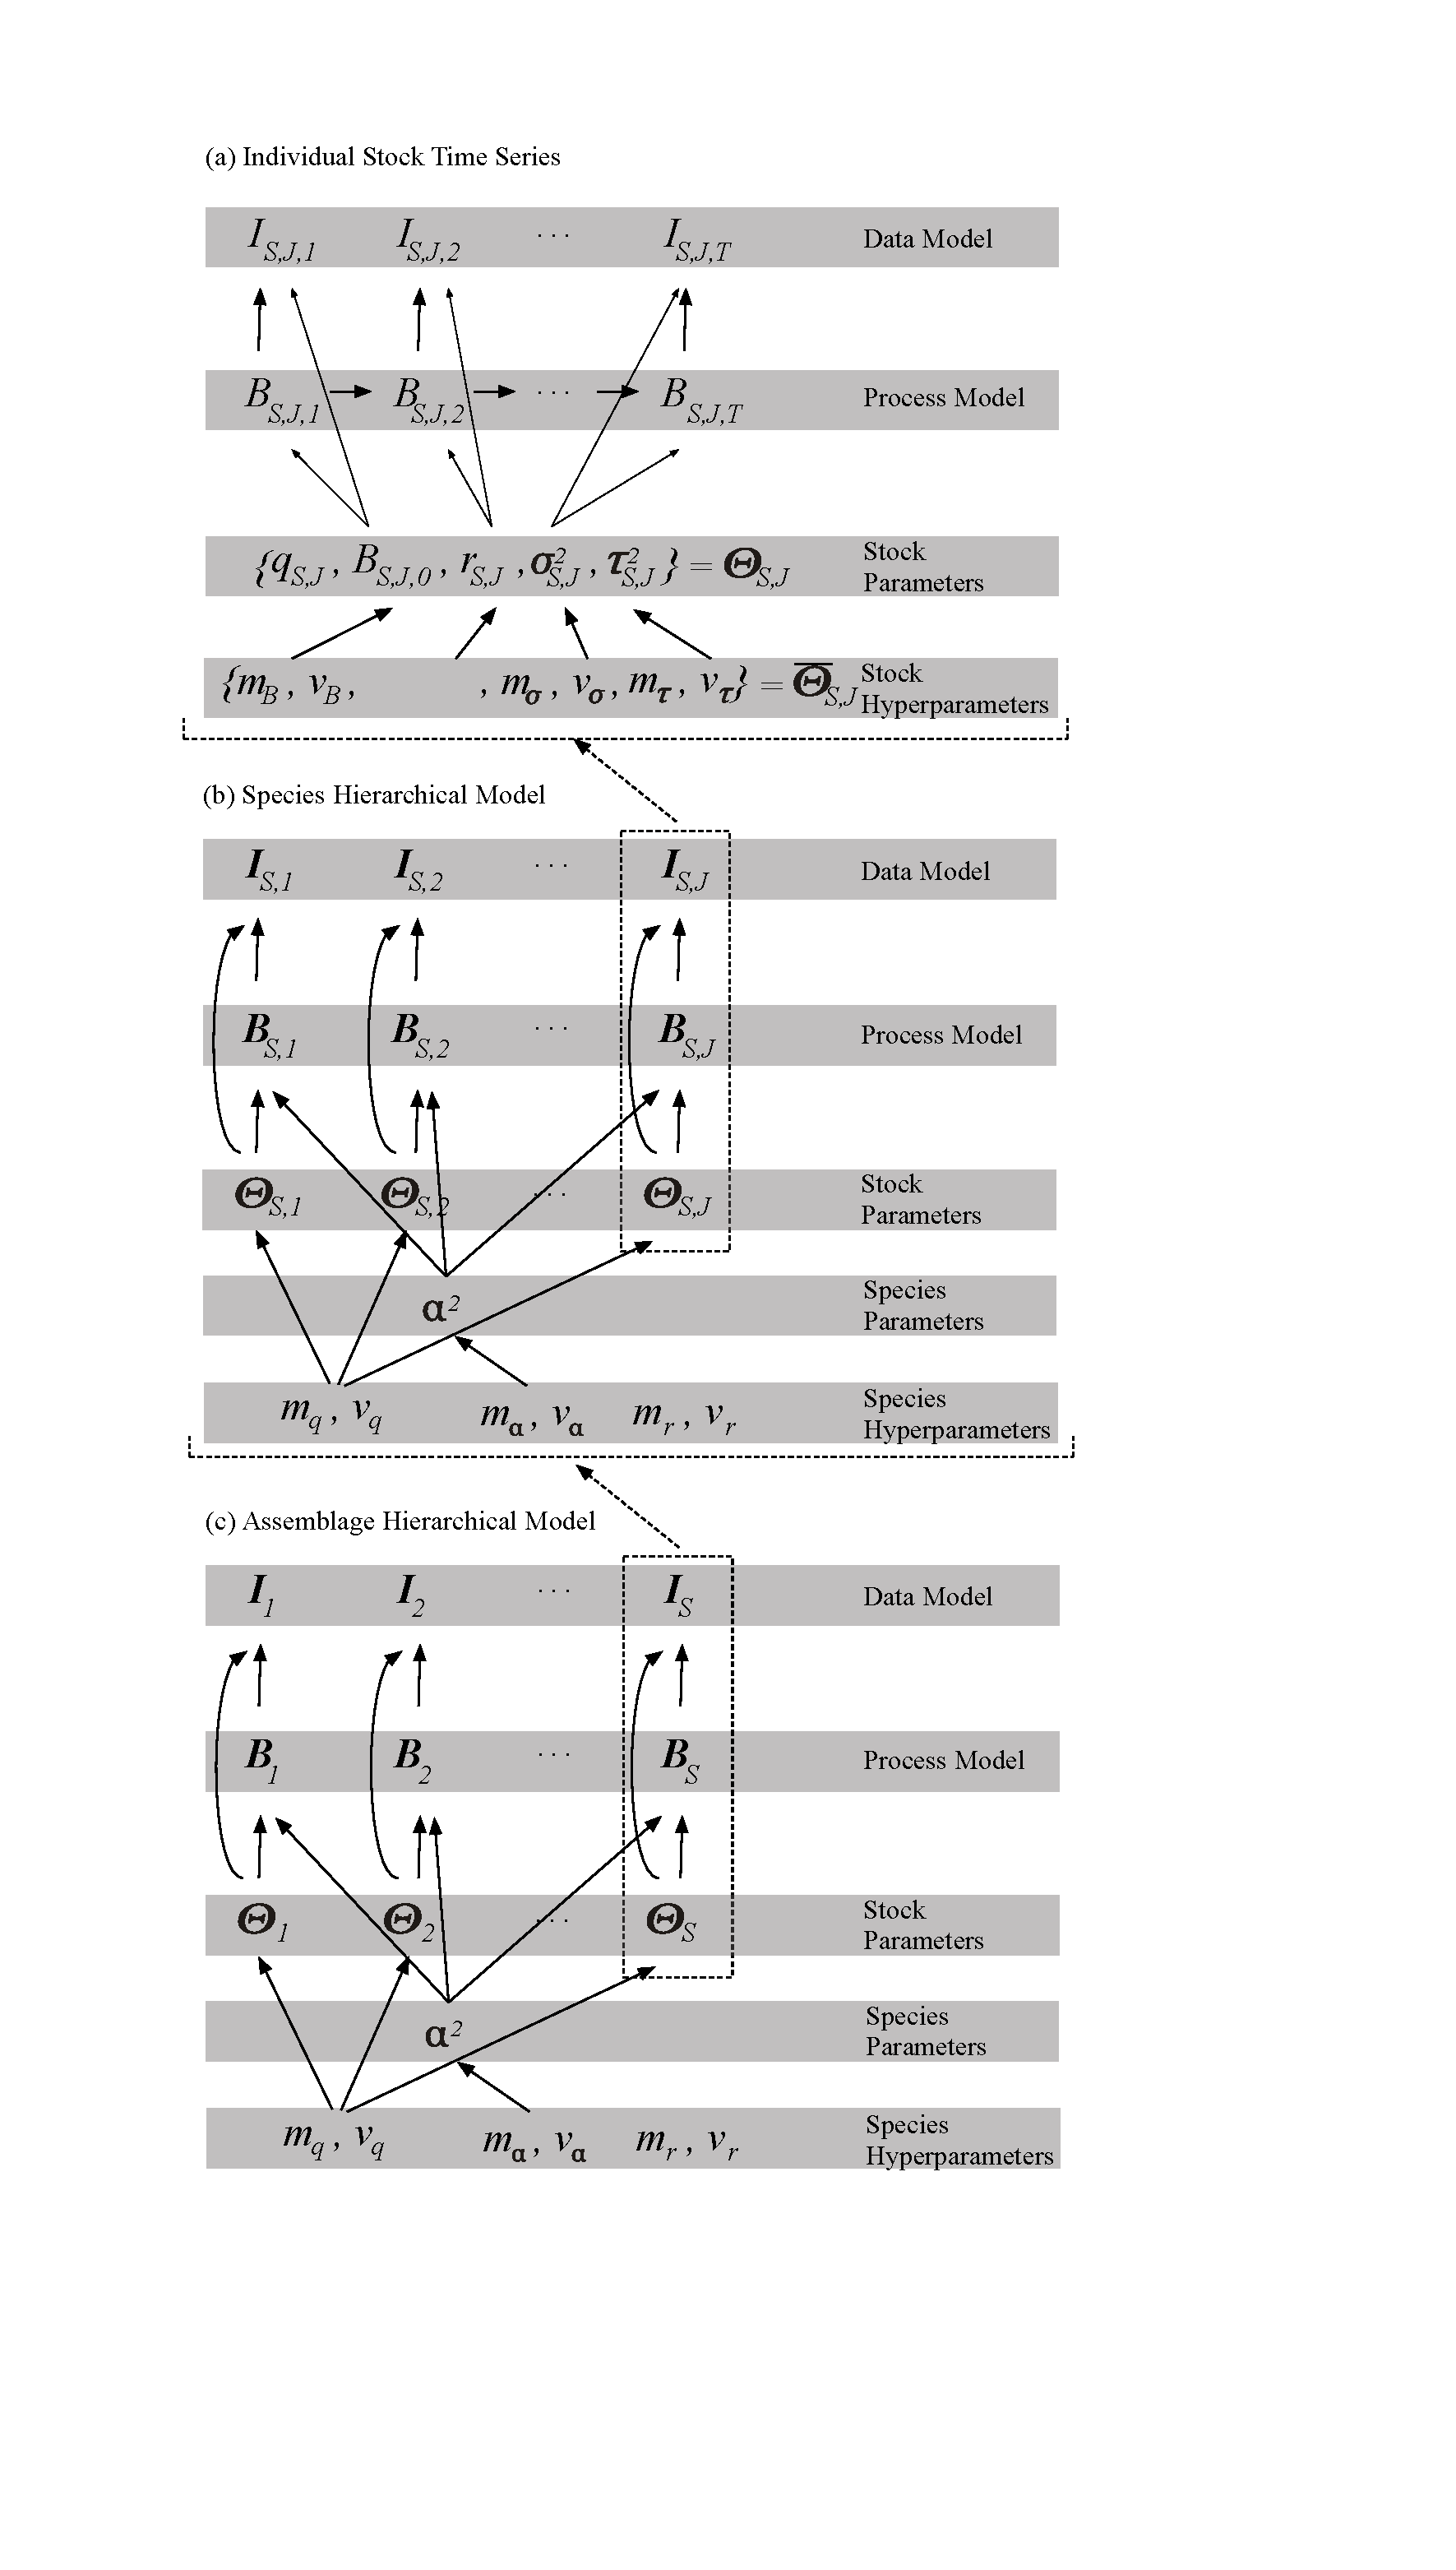
\includegraphics[scale = 0.4]{figures/HBMClarkCh2.pdf}
\caption{A conceptual diagram of the hierarchical model used for estimation in Chapter 2. Part (b) shows the hierarchically arranged species meta-population with species parameters and hyperparameters, where the time series in part (a) are compressed into bold, italicised symbols. Part (c) shows the hierarchically arranged multispecies assemblage, with shared multispecies parameters and hyperparameters.}\label{fig:HBMCh2}
\end{figure}

\newpage

\begin{table}[htbp]
\begin{center}
\caption{Variable definitions for the operating model simulation catch, effort, population dynamics and scientific observations in Chapter 3. The population dynamics are driven by a simple Biomass Dynamics model (Hilborn and Walters, 1992, Ch, 8), with immigration and emigration between stocks of a species summarised by a migration rate $\phi_{s,i,p}$. Catch is based on effort dynamics simulating targeting behaviour of harvesters.}\label{tab:OMspec}
\begin{tabular}{c|c}
\textit{Variable} & \textit{Description}  \\
\hline
& \textbf{ Index Variables} \\
\hline
$s$ & Species index \\
$p$ & Stock index \\
$f$ & Fleet index \\
$t$ & Time index \\
$S$ & Total number of species \\
$J_s$ & Total number of stocks of species $s$ \\
$F$ & Total number of fleets \\
$T$ & Total number of years \\
\hline
& \textbf{ Biological Model} \\
\hline
$B_{s,p,t}$ & Biomass of stock $p$ of species $s$ at time $t$ \\
$B_{s,p,0}$ & Unfished biomass of stock $p$ of species $s$ \\
$r_{s,p}$ & Intrinsic rate of growth for stock $p$ of speces $s$ \\
$\phi_{s,p,i}$ &  Net migration rate between stocks $p$ and $i$ of species $s$ \\
\hline
& \textbf{ Observation Model} \\
\hline
$q_{s,p}$ & Survey catchability of stock $p$ of species $s$ at time $t$ \\
$I_{s,p,t}$ & Fishery independent CPUE of stock $p$ of species $s$ at time $t$ \\
\hline
& \textbf{ Catch} \\
\hline
$E_{s,p,t,f}$ & Fishing effort expended by fleet $f$ to catch stock $p$ of species $s$ at time $t$ \\
$C_{s,p,t,f}$ & Total catch of stock $p$ of species $S$ at time $t$ by fleet $f$ \\
$C_{s,p,t}$ & Total catch of stock $p$ of species $S$ at time $t$ \\
$F_{s,p,t}$ & Fishing mortality of stock $p$ of species $s$ at time $t$ \\
\hline
& \textbf{ Stochastic Model } \\
$\sigma_{s,p}^2$ & Process error variance for stock $p$ of species $s$ \\
$\xi_{s,p,t}$ & Process error deviation for stock $p$ of species $s$ at time $t$, $\left( \epsilon_{s,p,t} \sim N (0, \sigma_{s,p}^2) \right)$ \\
$\sigma_{s}^2$ & Process error variance for species $s$ \\
$\zeta_{s,t}$ & Process error deviation for species $s$ at time $t$, $\left( \zeta_{s,t} \sim N (0, \sigma_s^2) \right)$ \\
$\sigma^2$ & Assemblage level process error variance  \\
$\epsilon_{t}$ & Assemblage level process error deviations at time $t$, $\left( \epsilon_{t} \sim N (0, \sigma^2) \right)$ \\
$\tau_s^2$ & Observation error variance for species $s$ \\
$\delta_{s,p,t}$ & Observation error for stock $p$ of species $s$ at time $t$ $\left(\epsilon_{s,p,t} \sim N (0, \tau_s^2) \right)$ \\
\hline
\end{tabular}
\end{center}
\end{table}

\newpage

\begin{figure}[htbp]
\centering
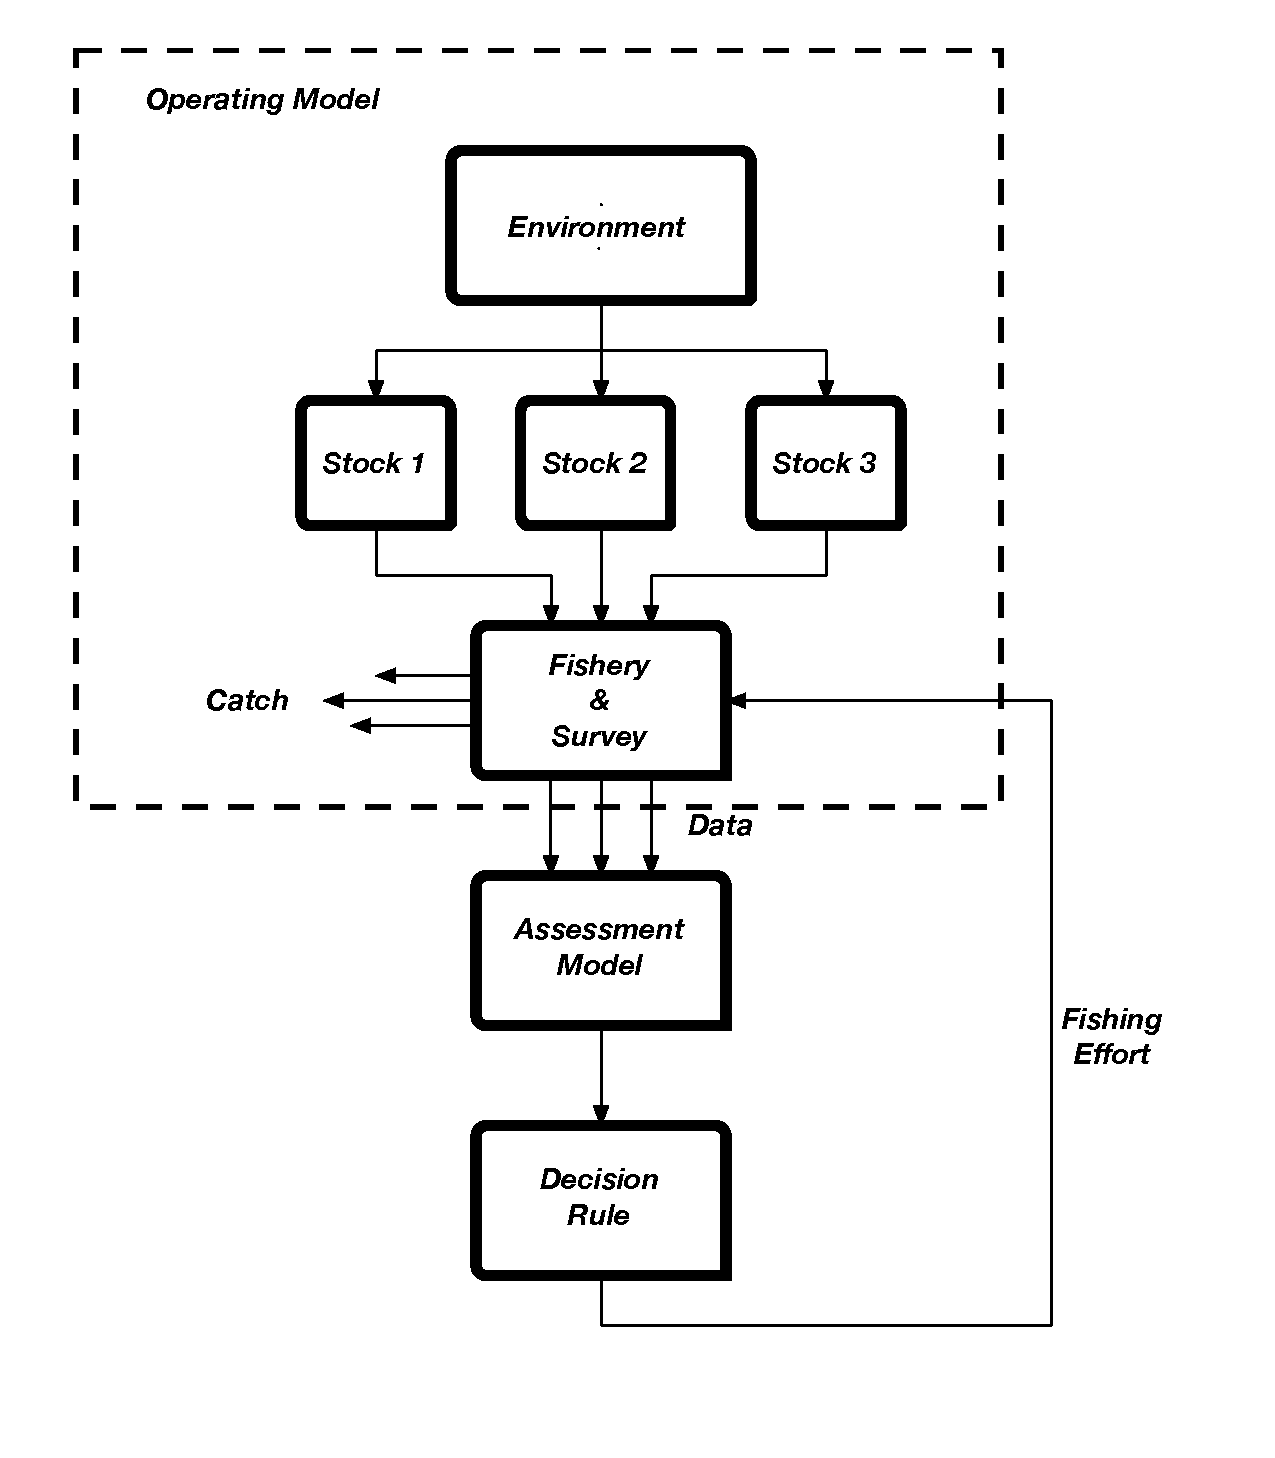
\includegraphics{figures/MSE.pdf}
\caption{A multi-species closed loop conceptual model. The operating model is oulined by the dashed line, which simulates three species with no sub-stock structure. Data generated by scientific observations and fishery exploitation at time step $t$ is provided to the assessment model. Assessment model output is passed through a decision rule, which provides catch advice for time step $t+1$. Fishing effort is then expended according to the catch advice, closing the loop and generating new data for the assessment model.}\label{fig:MSMSE}
\end{figure}\newpage

\begin{figure}[htbp]
\centering
\includegraphics{figures/ManagementAreas.pdf}
\caption{The 8 major statistical management areas of the BC integrated groundfish fishery.}\label{fig:statAreas}
\end{figure}\newpage

\begin{figure}[htbp]
\centering
\includegraphics{figures/sabComposition.pdf}
\caption{The top 15 species ranked by total catch weight (000s t) co-occurring in sets that caught Sablefish by bottom trawl gear from Jan 2009 to March 31, 2012 (left panel) and Apr 2012 to Mar 31, 2015 (right panel). Note that the bars for some top-ranked species have been truncated to fit on the plot; actual total catch weights are indicated to the right of the truncated bars for those species. This composition shows technical interactions between 3 DERPA species in trawl gear that encounters Sablefish.}\label{fig:catchComposition}
\end{figure}\newpage

\newpage

\begin{figure}[htbp]
\centering
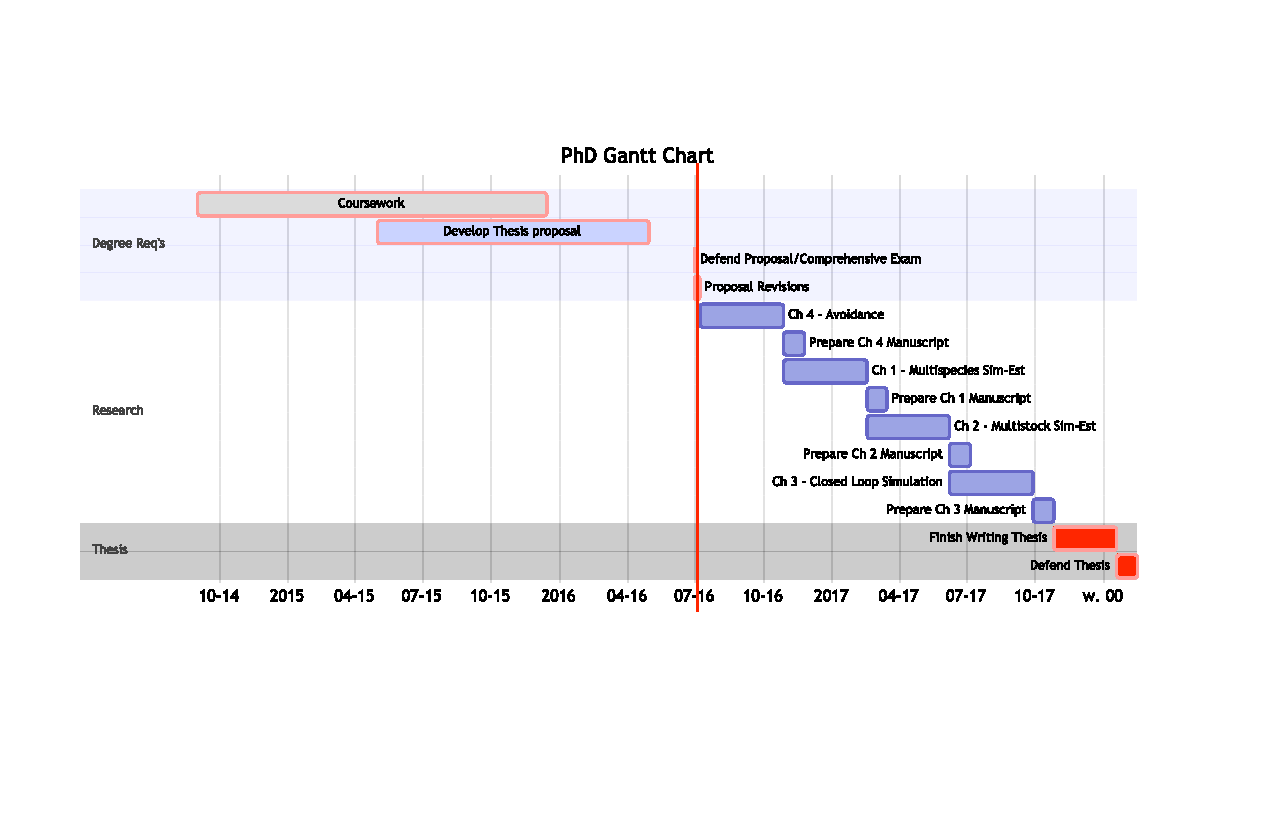
\includegraphics{figures/gantt.pdf}
\caption{A Gantt chart outlining the timeline of degree requirements, research, publications and thesis writing. Estimated time of completion is July 2018.}\label{fig:gantt}
\end{figure}

\end{document}